%-------------------------------------------------------------------------------
\section{Findings}
%-------------------------------------------------------------------------------

Due to the time and resources available for our experiment, our efforts were limited 
to four targets, \texttt{exiv2}, \texttt{infotocap}, \texttt{mp3gain}, and 
\texttt{tcpdump}\textbf{(RQ2)}. Each of these were included in Fu et al.\cite{fu_autofz_2023} 
and are part of

\substection(Autofz on AMD64)

Figure \ref{fig:exiv2_compare_orig_arm64} displays bitmap density covered by the individual algorithms in our AMD64 implementation, 
as compared to a similar plot from Fu et al.\cite{fu_autofz_2023}. While our recreation of autofz achieved lower bitmap coverage than 
the version published by Fu et al., our individual fuzzers also achieved lower bitmap coverage. As a result, our replica still 
outperformed all other individual fuzzers tested in our environment. This is consistant
with Fu et al.'s findings and further proves that \texttt{autofz} is superior to individual fuzzers.

\begin{figure}
    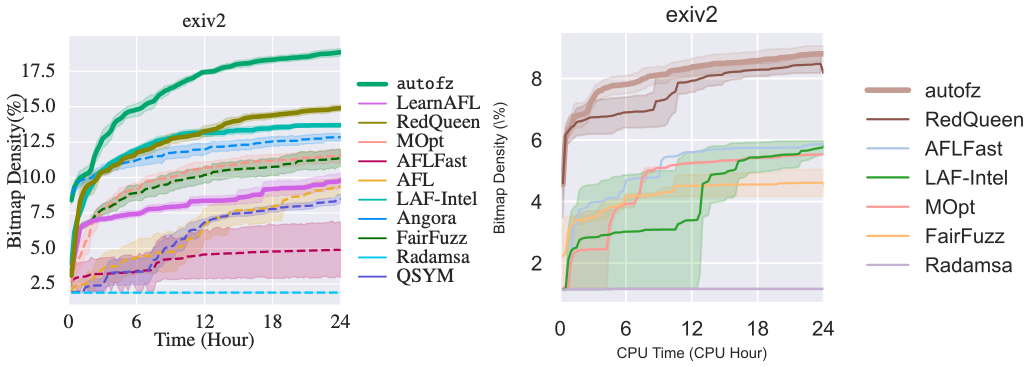
\includegraphics[width=0.52\textwidth]{figs/exiv2_compare_orig_arm64.png}
    \centering
    \caption{A comparison of bitmap density covered in the original\cite{fu_autofz_2023} and our 
    coverage during initial fuzzing of exiv2}
    \label{fig:exiv2_compare_orig_arm64}
\end{figure}

\substection(Autofz on ARM64)

Testing also indicates that the ARM64 compatible \texttt{autofz} performs similarly to the unmodified AMD64 \texttt{autofz}. 
Bitmap density coverage of AMD64 \texttt{autofz} is plottted alogside our ARM64 \texttt{autofz} in figure 
\ref{fig:tcpdump_compare_orig_arm64}. After 24 hours, both implementations achieved similar bitmap coverage.
AMD64 \texttt{Autofz}'s bitmap coverage grew linearly while ARM64 \texttt{autofz} followed a logarithmic trend. Consequently, 
the AMD64 \texttt{autofz} took longer to achieve the same bitmap coverage. 

\begin{figure}
    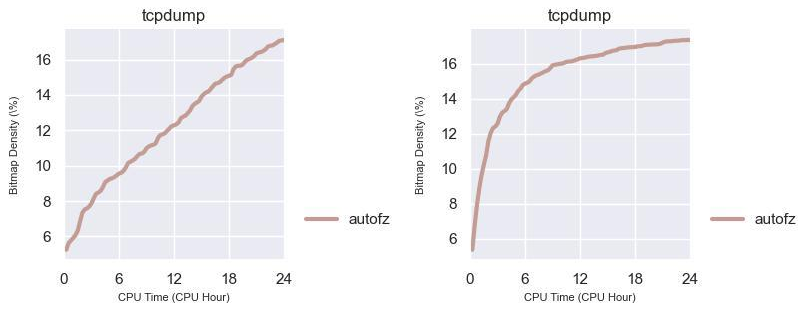
\includegraphics[width=0.52\textwidth]{figs/tcpdump_compare_orig_arm64.png}
    \centering
    \caption{A comparison of bitmap density covered in AMD64 \texttt{autofz} and our ARM64 implementation
    coverage during fuzzing of tcpdump}
    \label{fig:tcpdump_compare_orig_arm64}
\end{figure}

Bug coverage of our ARM64 fuzzing campaign against tcpdump is plotted in figure \ref{figs:tcp_compare_orig_arm64_ub.png}, 
shown as a comparison are results from Fu et al.\cite{fu_autofz_2023}. While the ARM64 adaptation of \texttt{autofz} achieved similar
performance to the original in bitmap coverage, it out performed the original in bug discovery. Since the other targets followed similar trends
when fuzzed with ARM64 \texttt{autofz}, \texttt{autofz} can be successfully adapted for the ARM64 architecture.

\begin{figure}
    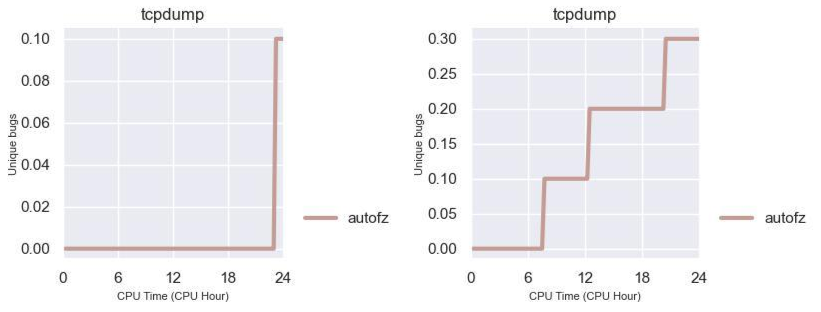
\includegraphics[width=0.52\textwidth]{figs/tcpdump_compare_orig_arm64_ub.png}
    \centering
    \caption{A comparison of bug discovery in AMD64 \texttt{autofz} and our ARM64 implementation
    coverage during fuzzing of tcpdump}
    \label{figs:tcp_compare_orig_arm64_ub.png}
\end{figure}

\substection(Additional Metrics for Autofz)

The outcomes of the new resource allocation algorithms on tcpdump in ARM64 and AMD64 are documented in \ref{figs:tcpdump_algo_compare.png}. 
The outcomes of these algorithms were not consistent. While the ub-bitmap algorithm outperforms the others when tested on the AMD64, a 
consistent winner does not present when the algorithms are tested in the ARM64 envirnoment. 

\begin{figure}
    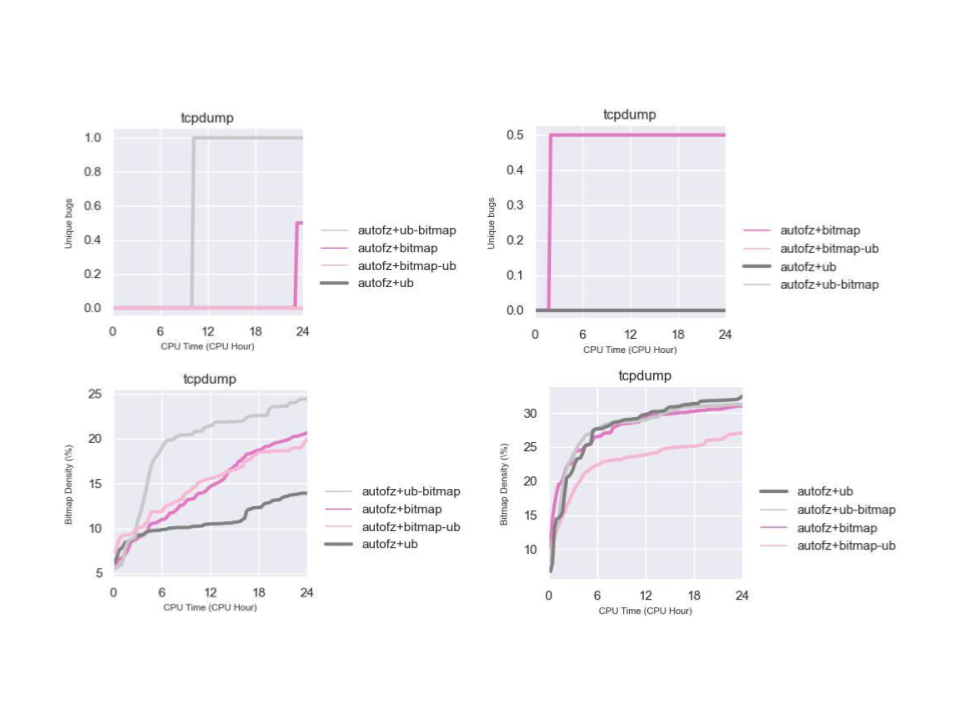
\includegraphics[width=0.52\textwidth]{figs/tcpdump_algo_compare.png}
    \centering
    \caption{The outcomes of the new resource allocation algorithms on tcpdump when executed on the AMD64 and ARM64 architectures}
    \label{figs:tcpdump_algo_compare.png}
\end{figure}

The inverse of this pattern can be identifed when the new resource allocation algoritions are executed on infotocap in 
\ref{figs:infotocap_algo_compare.png}. When the new algorithms are tested on infotocap in AMD64 \testtt{autofz}, one does not achieve better
bitmap coverage and bug discovery, but when the new algorithms are tested on ARM64 \testtt{autofz}, ub-bitmap is the best algorithm.

\begin{figure}

    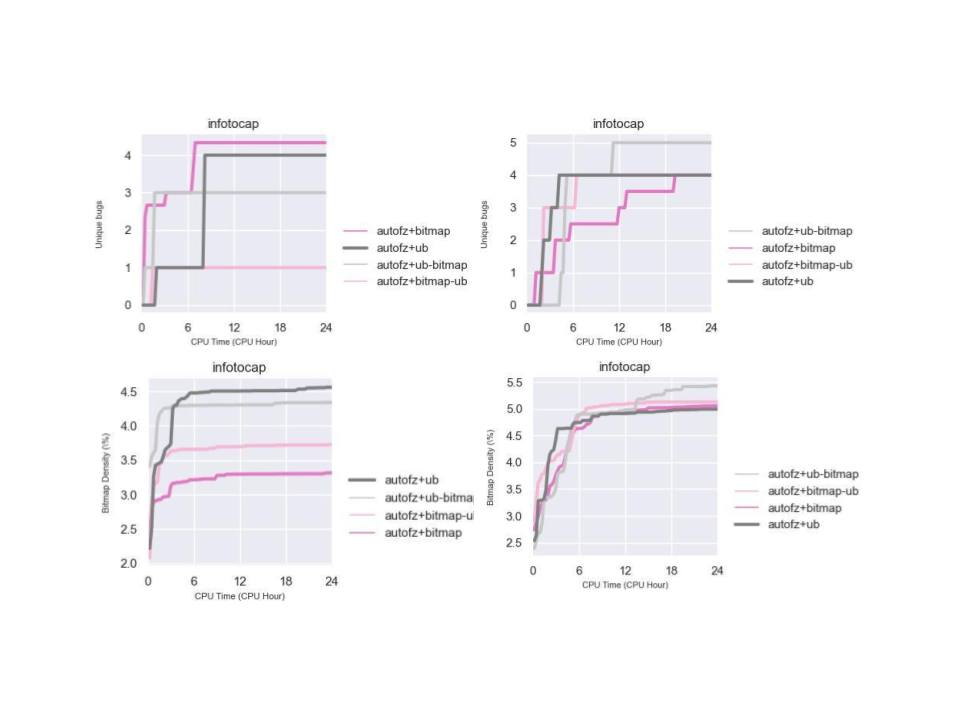
\includegraphics[width=0.52\textwidth]{figs/infotocap_algo_compare.png}
    \centering
    \caption{The outcomes of the new resource allocation algorithms on infotocap when executed on the AMD64 and ARM64 architectures}
    \label{figs:infotocap_algo_compare.png}
\end{figure}

As a result of these inconsistencies, one algorithm cannot be identifed as better than the others at this time.


